\subsection{Núcleo Andromeda: Comunicação de Engajamento}

\begin{figure}[!htbp]
\centering
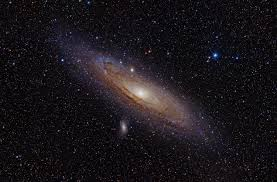
\includegraphics[width=1\linewidth]{files/andromeda-24292683f0310a3e603bd61d6d950606.jpeg}
\end{figure}

\subsubsection{Visão Geral}

O \textbf{Núcleo Andromeda} é responsável pela comunicação de engajamento digital do Projeto Hermathena. Seu nome evoca a galáxia vizinha, simbolizando a expansão e alcance da mensagem do BINGO através das redes sociais e canais digitais.

\subsubsection{Missão}

Criar conexões emocionais e intelectuais entre o público e o Radiotelescópio BINGO através de conteúdo digital criativo, acessível e viral, construindo uma comunidade online engajada em torno da ciência.

\subsubsection{Objetivos Específicos}

\paragraph{1. Gestão de Redes Sociais}

\subparagraph{1.1 Instagram}

\begin{itemize}
\item[$\square$] Criar e manter perfil oficial do Projeto Hermathena/BINGO PB
\item[$\square$] Publicar feed diário com conteúdo variado
\item[$\square$] Produzir Stories com interatividade (enquetes, caixinhas de perguntas)
\item[$\square$] Desenvolver Reels virais sobre astronomia e cosmologia
\item[$\square$] Alcançar 5.000 seguidores no primeiro ano
\item[$\square$] Manter taxa de engajamento superior a 5\%
\end{itemize}

\subparagraph{1.2 Facebook}

\begin{itemize}
\item[$\square$] Manter página institucional atualizada
\item[$\square$] Criar grupo de comunidade para educadores
\item[$\square$] Compartilhar eventos e lives
\item[$\square$] Publicar conteúdo em formato de álbum
\item[$\square$] Interagir com páginas de parceiros
\end{itemize}

\subparagraph{1.3 TikTok}

\begin{itemize}
\item[$\square$] Criar perfil com identidade jovem e descontraída
\item[$\square$] Produzir vídeos curtos (15-60 segundos)
\item[$\square$] Participar de trends educativas
\item[$\square$] Criar desafios de ciência
\item[$\square$] Colaborar com criadores de conteúdo da região
\end{itemize}

\paragraph{2. Estratégias de Conteúdo}

\subparagraph{2.1 Formatos por Plataforma}

\bigskip\noindent
\begin{tabular}{p{\dimexpr 0.250\linewidth-2\tabcolsep}p{\dimexpr 0.250\linewidth-2\tabcolsep}p{\dimexpr 0.250\linewidth-2\tabcolsep}p{\dimexpr 0.250\linewidth-2\tabcolsep}}
\toprule
Plataforma & Formato Principal & Frequência & Tom \\
\hline
Instagram & Carrossel educativo & Semanal & Inspirador \\
Instagram & Reels & Semanal & Entretenimento \\
Stories & Interativo & Semanal & Conversacional \\
Facebook & Posts longos & Semanal & Informativo \\
TikTok & Vídeos curtos & Semanal & Descontraído \\
\bottomrule
\end{tabular}

\bigskip

\subparagraph{2.2 Linhas Editoriais}

\textbf{\#CosmoEm60Segundos}

\begin{itemize}
\item Explicações rápidas de conceitos astronômicos
\item Curiosidades do universo
\item Respostas a perguntas do público
\end{itemize}

\textbf{\#BINGONoDetalhe}

\begin{itemize}
\item Bastidores da construção do telescópio
\item Entrevistas com técnicos e engenheiros
\item Mostra de equipamentos e tecnologia
\end{itemize}

\textbf{\#ParaibaNoEspaco}

\begin{itemize}
\item Conexão entre o Sertão e a cosmologia
\item Histórias de pessoas do projeto
\item Beleza do Vale do Piancó
\end{itemize}

\textbf{\#DesafioSTEM}

\begin{itemize}
\item Experimentos caseiros de ciência
\item Desafios para estudantes
\item Quiz e perguntas interativas
\end{itemize}

\textbf{\#CienciaNaPratica}

\begin{itemize}
\item Vídeos de demonstrações
\item Lives de observação astronômica
\item Eventos em tempo real
\end{itemize}

\paragraph{3. Produção de Conteúdo Viral}

\subparagraph{3.1 Biblioteca de Conteúdo}

\bigskip\noindent
\begin{tabular}{p{\dimexpr 0.333\linewidth-2\tabcolsep}p{\dimexpr 0.333\linewidth-2\tabcolsep}p{\dimexpr 0.333\linewidth-2\tabcolsep}}
\toprule
Tipo & Quantidade Anual & Exemplos \\
\hline
Infográficos & 12 & ``O que são BAO?'', ``Escala do Universo'' \\
Vídeos curtos & 50 & Reels, TikToks, Shorts \\
Memes educativos & 30 & Astronomia em formato humor \\
\bottomrule
\end{tabular}

\bigskip

\subparagraph{3.2 Série Regular ``BINGO Responde''}

Formato: Vídeos curtos respondendo perguntas do público

\begin{itemize}
\item Duração: 30-60 segundos
\item Frequência: Semanal
\item Call-to-action: ``Mande sua pergunta nos comentários''
\end{itemize}

\paragraph{4. Engajamento Comunitário}

\subparagraph{4.1 Estratégias de Interação}

\begin{itemize}
\item \textbf{Responder todos os comentários} em até 12 horas
\item \textbf{Compartilhar posts de seguidores} que mencionarem o projeto
\item \textbf{Criar desafios mensais} com premiação simbólica
\item \textbf{Live quinzenal} com especialistas (colaboração com Núcleo Triangulum)
\end{itemize}

\subparagraph{4.2 Parcerias com Influenciadores}

\bigskip\noindent
\begin{tabular}{p{\dimexpr 0.333\linewidth-2\tabcolsep}p{\dimexpr 0.333\linewidth-2\tabcolsep}p{\dimexpr 0.333\linewidth-2\tabcolsep}}
\toprule
Categoria & Perfil & Ação \\
\hline
Educação & Professores de ciências & Divulgação em sala \\
Lifestyle & Criadores da Paraíba & Visita ao BINGO \\
Ciência & Divulgadores científicos & Colaboração de conteúdo \\
Local & Prefeituras da região & Alcance institucional \\
\bottomrule
\end{tabular}

\bigskip

\paragraph{5. Monitoramento e Métricas}

\subparagraph{5.1 KPIs Principais}

\bigskip\noindent
\begin{tabular}{p{\dimexpr 0.333\linewidth-2\tabcolsep}p{\dimexpr 0.333\linewidth-2\tabcolsep}p{\dimexpr 0.333\linewidth-2\tabcolsep}}
\toprule
Indicador & Meta Ano 1 & Ferramenta \\
\hline
Seguidores Instagram & 5.000 & Insights nativo \\
Seguidores TikTok & 3.000 & TikTok Analytics \\
Taxa de engajamento & \textgreater 5\% & Metricool/Sprout \\
Alcance mensal & 100.000 & Meta Business \\
Compartilhamentos & 1.000/mês & Analytics \\
Saves (Instagram) & 500/mês & Insights nativo \\
\bottomrule
\end{tabular}

\bigskip

\subparagraph{5.2 Relatórios}

\begin{itemize}
\item \textbf{Semanal:} Métricas rápidas de performance
\item \textbf{Mensal:} Análise detalhada com insights
\item \textbf{Trimestral:} Relatório completo para coordenação
\end{itemize}

\subparagraph{5.3 Ferramentas de Gestão}

\begin{itemize}
\item \textbf{Agendamento:} Metricool ou Later
\item \textbf{Design:} Canva Pro + Adobe Creative Cloud
\item \textbf{Edição de vídeo:} CapCut + Premiere Pro
\item \textbf{Analytics:} Meta Business Suite, TikTok Analytics
\end{itemize}

\subsubsection{Metodologia}

\paragraph{Fluxo de Produção de Conteúdo}

\begin{verbatim}
flowchart LR

A["Planejamento"]
B["Produção"]
C["Agendamento"]
E["Publicação"]
D["Análise"]

A - -> B - -> C
C - -> E
E - -> D
D - -> A

classDef p fill:#ff9a6e,color:white;
classDef prod fill:#F54927,color:white;
classDef exec fill:#c53a1f,color:white;
classDef anal fill:#8e2415,color:white;

class A p
class B,C prod
class E exec
class D anal
\end{verbatim}

\paragraph{Processo de Criação}

\begin{enumerate}
\item \textbf{Briefing} - Definição de objetivo, público e formato
\item \textbf{Pesquisa} - Verificação de dados científicos
\item \textbf{Roteirização} - Texto e estrutura visual
\item \textbf{Produção} - Design e edição
\item \textbf{Revisão} - Validação com equipe científica
\item \textbf{Aprovação} - Coordenação final
\item \textbf{Publicação} - Postagem otimizada
\item \textbf{Monitoramento} - Acompanhamento de performance
\end{enumerate}

\subsubsection{Cronograma de Ações (Ano 1)}

\bigskip\noindent
\begin{tabular}{p{\dimexpr 0.250\linewidth-2\tabcolsep}p{\dimexpr 0.250\linewidth-2\tabcolsep}p{\dimexpr 0.250\linewidth-2\tabcolsep}p{\dimexpr 0.250\linewidth-2\tabcolsep}}
\toprule
Trimestre & Ação & Responsável & Produto \\
\hline
\textbf{T1} & Setup dos perfis & Equipe & Perfis criados e configurados \\
\textbf{T1} & Definição de identidade visual digital & Designer & Guia de uso em redes sociais \\
\textbf{T2} & Produção de 30 posts iniciais & Equipe & Biblioteca de conteúdo \\
\textbf{T2} & Primeiras lives & Equipe & 4 transmissões ao vivo \\
\textbf{T3} & Campanha de crescimento & Equipe & Meta: 2.000 seguidores \\
\textbf{T3} & Parcerias com influencers & Coordenação & 3 colaborações \\
\textbf{T4} & Análise e otimização & Equipe & Relatório de melhores práticas \\
\textbf{T4} & Planejamento ano 2 & Coordenação & Calendário editorial anual \\
\bottomrule
\end{tabular}

\bigskip

\subsubsection{Campanhas Temáticas}

\paragraph{Calendário de Campanhas}

\bigskip\noindent
\begin{tabular}{p{\dimexpr 0.250\linewidth-2\tabcolsep}p{\dimexpr 0.250\linewidth-2\tabcolsep}p{\dimexpr 0.250\linewidth-2\tabcolsep}p{\dimexpr 0.250\linewidth-2\tabcolsep}}
\toprule
Mês & Campanha & Tema & Hashtag \\
\hline
Março & Dia da Astronomia & Mulheres na astronomia & \#MulheresNoBINGO \\
Abril & Semana da Terra & Terra e cosmologia & \#TerraNoCosmos \\
Maio & Dia do Astronauta & Exploração espacial & \#ParaibaNoEspaco \\
Junho & Dia do Meio Ambiente & Radioastronomia e preservação & \#BINGOVerde \\
Agosto & Dia do Estudante & Carreiras STEM & \#FuturoBINGO \\
Setembro & Semana Nacional de Ciência & Divulgação massiva & \#BINGOCiencia \\
Outubro & Dia das Crianças & Astronomia para pequenos & \#BINGOKids \\
Novembro & ENEM & Ciência na Escola & \#BINGOENEM \\
Dezembro & Retrospectiva & Melhores momentos do ano & \#BINGO2026 \\
\bottomrule
\end{tabular}

\bigskip

\subsubsection{Estrutura da Equipe}

\bigskip\noindent
\begin{tabular}{p{\dimexpr 0.333\linewidth-2\tabcolsep}p{\dimexpr 0.333\linewidth-2\tabcolsep}p{\dimexpr 0.333\linewidth-2\tabcolsep}}
\toprule
Função & Quantidade & Perfil \\
\hline
\textbf{Professor Orientador} & 1 & Docente Comunicação/Educomunicação \\
\textbf{Professor Colaborador} & 1 & Docente arte/mídia/jornalismo \\
\textbf{Bolsista PROBEX} & 1 & Graduação Comunicação/Jornalismo \\
\textbf{Voluntários} & 5 & Graduação em áreas afins \\
\bottomrule
\end{tabular}

\bigskip

\textbf{Total por núcleo:} 8 pessoas

\textbf{Expansão:} Pode replicar em instituições parceiras (até 12 alunos + 4 docentes)

\subsubsection{Orçamento Estimado (Ano 1)}

\bigskip\noindent
\begin{tabular}{p{\dimexpr 0.500\linewidth-2\tabcolsep}p{\dimexpr 0.500\linewidth-2\tabcolsep}}
\toprule
Categoria & Valor (R\$) \\
\hline
Bolsa (1 bolsista $\times$ 6 meses $\times$ R\$ 400) & 2.400,00 \\
Assinaturas de ferramentas & 3.600,00 \\
Equipamentos (ring light, tripé) & 2.000,00 \\
Eventos e parcerias & 3.000,00 \\
\textbf{Total} & \textbf{28.000,00} \\
\bottomrule
\end{tabular}

\bigskip

\subsubsection{Benchmarking}

\paragraph{Referências em Comunicação Científica Digital}

\bigskip\noindent
\begin{tabular}{p{\dimexpr 0.333\linewidth-2\tabcolsep}p{\dimexpr 0.333\linewidth-2\tabcolsep}p{\dimexpr 0.333\linewidth-2\tabcolsep}}
\toprule
Projeto & Plataforma & O que aprender \\
\hline
\cite{AstroPocket} & Instagram & Formato de carrossel educativo \\
\cite{CanalNostalgia} & YouTube/Instagram & Como viralizar ciência \\
NASA & Todas & Estratégia multicanal \\
IFScience & Facebook & Engajamento com conteúdo leve \\
Manual do Mundo & YouTube & Produção de vídeos didáticos \\
\bottomrule
\end{tabular}

\bigskip


\bigskip
\centerline{\rule{13cm}{0.4pt}}
\bigskip

\textit{Documento sujeito a revisões conforme evolução das plataformas digitais.}